\pagebreak
\subsection{Software Design}
\subsubsection{Purpose}
The purpose of the software is to automatically control the valves so that they will be opened/closed at the designated altitude. Moreover, the software will store housekeeping data from sensors, pump and valves states to the on-board memory storage device. To determine a vertical profile, the acquisition of sensor data is required. From Olivier's research:
\begin{quote}
"In order to determine the vertical profiles of CO$_2$ and CH$_4$ from the analysis of sampled air, measurements of several atmospheric parameters are needed (see Sect. 2.3). The two most important parameters are the ambient pressure and the mean coil temperature. Those parameters are recorded by the AirCore-HR electronic data package. Mean coil temperature is obtained by taking the mean of three temperatures recorded by independent probes located at different positions along the AirCore-HR".\cite{Olivier}
\end{quote}
The next purpose is to transmit such data to the ground. It will allow the team to monitor the real-time condition of the experiment. Telecommand is also needed to take over the experiment if the software automation fails, since this experiment is highly dependent on the software. It will also be used to test the system, especially valves and heaters.\par
\subsubsection{Design}
\begin{enumerate}[label=(\alph*)]
\item{Process Overview}\\
The software which run on the Arduino reads from the sensors through the I2C and SPI interfaces. The sensors provides temperature, pressure, airflow and humidity data. The acquired data will be time-stamped and stored on the on-board SDcard and transmitted via the E-Link System to the ground station. Then according to the pressure/altitude, the software controls the valves which will allow the air to flow inside the tube and bags. Figure \ref{processOverview} visually explain the process flow.
\begin{figure}[H]
    \centering
    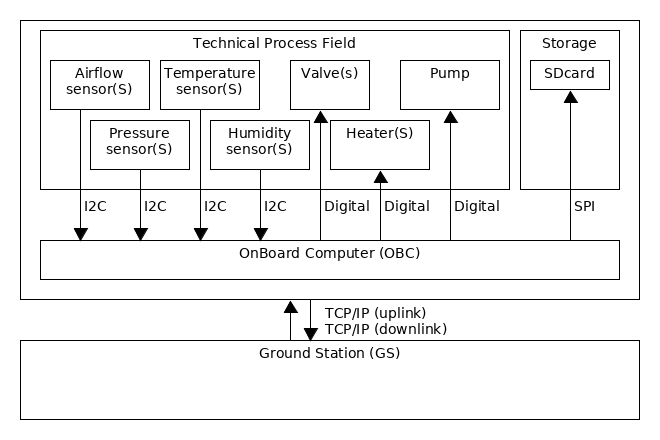
\includegraphics[width=0.85\textwidth]{4-experiment-design/img/Process-overview-V0-1.png}
    \caption{The process overview of the experiment}
    \label{processOverview}
\end{figure}
\item{General and Safety related concepts}\\
Watchdog timer, which is an electronic countdown timer that causes an interrupt when it reaches 0, will be used to avoid failure because of a freezing software. During normal operations, the software will regularly reset the the watchdog timer to prevent it from elapsing, or \enquote{timing out}. Telecommands will also be used as backup in case the automation fails or otherwise become unresponsive. Telemetry will be utilized to transmit housekeeping data and the state of the valves to get conformation of operation. Rigorous testing will be performed during the development of the project and before the launch phase to insure that that the software is capable to control the experiment. Watchdog implementation will be finalized after further test.
\item{Interfaces}\\
Table \ref{tab:comIntpro} demonstrates how the components will interact with the onboard computer (OBC). Components that use SPI, will share MISO, MOSI, and CLK pins on the Arduino board. Each of them will also be connected to general pins input output (GPIO) for slave select. Furthermore, components using I2C protocol, will share Serial Data pin (SDA) and Serial Clock pin (SCL).

\begin{table}[H]
\centering
\begin{tabular}{lll}
Components interacting & Communication protocol & Interface                 \\ \hline
Pressure Sensors-OBC   & SPI                    & Arduino SPI and Digital Pins \\
Temperature sensors-OBC        & I2C                    & Arduino I2C \\
Airflow sensor-OBC     & I2C                    & Arduino I2C \\
Heaters-OBC            & Digital                & GPIO pins \\
Air pump-OBC           & Digital                & GPIO pins \\
Valve-OBC              & Digital                & GPIO pins                 \\
OBC-microSD Storage    & SPI                    & Arduino Ethernet shield   \\
OBC - E-Link           & Ethernet               & Ethernet port            
\end{tabular}%Tabular dude
\caption{Communication and interface protocols}
\label{tab:comIntpro}
\end{table}

Every transmission to/from the ground will utilize the E-link connection. The data packet which will be used is Ethernet Packet with a header contains the address of destination, followed by the data, and at the end there is a frame check sequence (FCS). The up-linked data packet will have the same structure, with header followed by commands and ended with FCS.\\
\\
The protocol that has been chosen are UDP for telemetry and TCP for telecommand. The UDP is used to prevent software getting stuck waiting for handshake from the ground if the connection is temporarily lost.
\item{Data Acquisition and Storage}\\
Data will be stored on the SD memory card on the Arduino Ethernet Shield. It is estimated that for the entire flight, all the sensors will produce $4.896$ MB of data. The sampling rate will be fixed at 2 sampling per second.\\
\\
The data will be collected and presented as a matrix, where the first column is the time frame, the following columns are the sensors data. After the sensors data, there will also be housekeeping data, that keeps track of the valves, and heaters states. However, the size of the housekeeping data is not expected to surpass 20 bits per sampling.\\
\\
Data will be continuously down-linked 2 times per second and the total telemetry size is $7.128$ MB for 10 hours of flight. On the other hand, the telecommand size will vary based on how many subcommand is sent each time. If all of the subcommand are enabled, the total size is 128 bytes. Considering the telecommand will not be sent more than once per second, the telecommand data rate is 126 bytes/sec.
\item{Process Flow}\\
The process flow can be explained with the mode diagram in figure \ref{fig:modediag}. The software will start with Standby Mode, in which the software will get samples from all sensors. The on-board memory card contains the default sampling schedule parameters (when the sampling will start and stop), which will be read by the software in Standby Mode. When the software got reading of pressure changes (decrease), it will change to Normal - Ascent mode, where the software will empty the tube and bags by opening the valves. Then, at certain altitudes, air sampling will be conducted during ascending phase. During floating phase, there will be nothing conducted. The software will go to Normal - Descent mode when it sense when the pressure reduction is considerably big, where the software will sample the air by opening the valves for each bag in their designated altitude. The air sampling during descent phase will only be started after the gondola stabilize after cut-off. The software will know this by the reduction of pressure value readings. The experiment goes to SAFE mode between $5$ to $10 \, km$ before the landing, where all the valves will be closed. 
\begin{figure}[H]
    \begin{align*}
        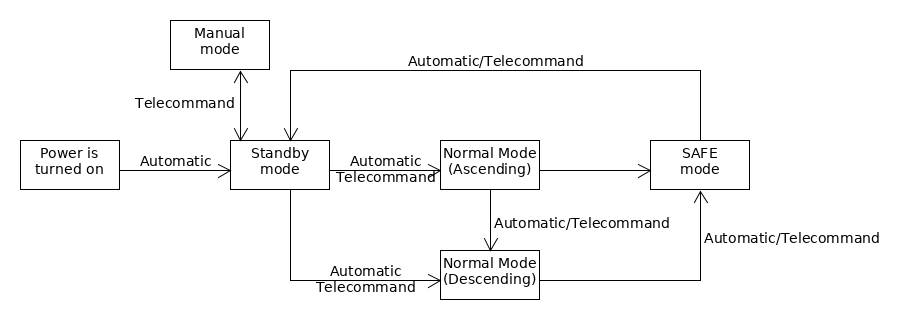
\includegraphics[width=1\linewidth]{4-experiment-design/img/state-diagram-V1-2.png}
    \end{align*}
    \caption{Process diagram for the modes}\label{fig:modediag}
\end{figure}
\item{Modularization and Pseudo Code}\\
\begin{figure}[H]
    \begin{align*}
        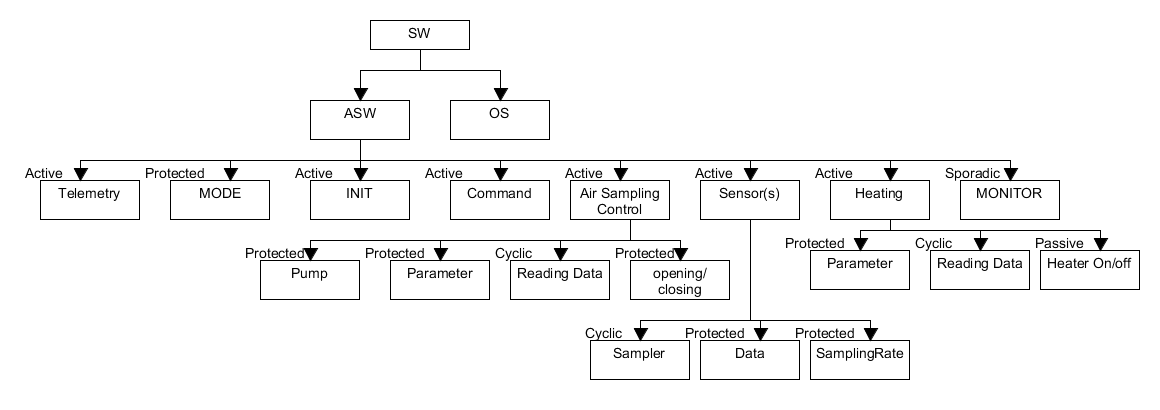
\includegraphics[width=1\linewidth]{4-experiment-design/img/sw_design.png}
    \end{align*}
    \caption{Onboard Software Design Tree}\label{fig:obtree}
\end{figure}
The software design is produced by using object oriented approach. The functionality of the experiment has been divided into several objects and their children. The design tree is shown in Figure \ref{fig:obtree}.\\
\\
The Telemetry object is responsible to format the sensor/housekeeping data, and to transmit it. MODE is responsible for controlling the four modes of software. INIT will initialize the necessary software programs. COMMANDS reads the telecommands and execute their commands. The AIR SAMPLING CONTROL object have the four children objects. The first child is responsible for controlling the pump. The second child contains the parameters for the valves and pump. The third child reads the data from the sensors, a fourth child is responsible for manipulating the valves.\\
\\
The SENSOR object have two children objects. One for sampling the sensors and another for recording and storing the housekeeping data. The HEATER object have three children objects. One for reading the temperature sensor data, another for deciding if the heaters should be turn on/off. And the third child for turning it on/off.\\ 
\\
Each of the objects interacts with each others fulfilling mutually exclusive interaction. It means that any shared variables can only be accessed by one object at time. This is important considering the program is be fully automatic and to prevent unnecessary data lost. The objects interface diagrams and their sequence diagrams can be found in Appendix \ref{sec:appB} and \ref{sec:appC}.
\end{enumerate}
%\begin{figure}[H]
%    \centering
%    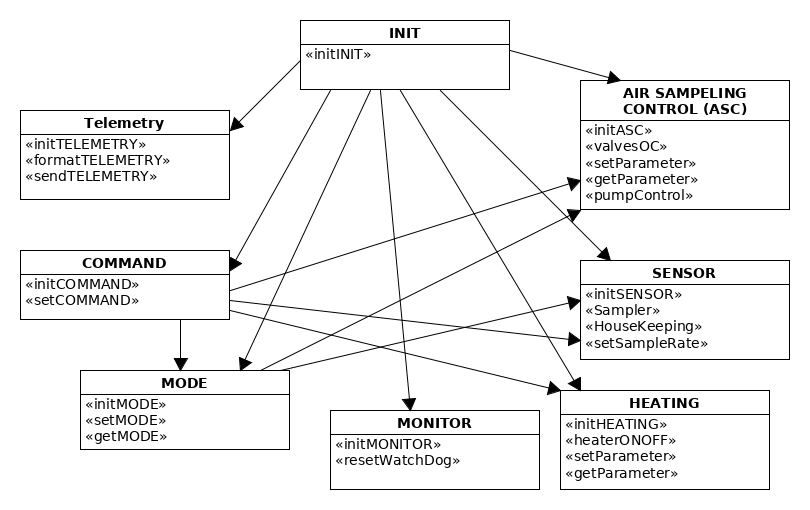
\includegraphics[width=1\textwidth]{4-experiment-design/img/hood-diagram-v1-0.png}
%    \caption{Hierarchic Object-Oriented Design of the software}
%    \label{fig:hood}
%\end{figure}
\subsubsection{Implementation}
The C/C++ programming language is used when programming the platform. Software's as PlatformIO IDE is used, other software will be used if necessary. FreeRTOS is chosen as the real-time operating system, this allowed us to split functionality into several mutual exclusive tasks. Several libraries that are used:
\begin{itemize}
    \item FreeRTOS\_ARM.h (FreeRTOS specially port for ARM microprocessor like Due)
    \item ArduinoSTL.h (allows standard C++ functionality)
    \item Necessary Arduino libraries.
    \item Sensors libraries.
\end{itemize}


\raggedbottom